\subsection{Niveau 2 - Détecter}

\begin{center}
\begin{figure}[!h]
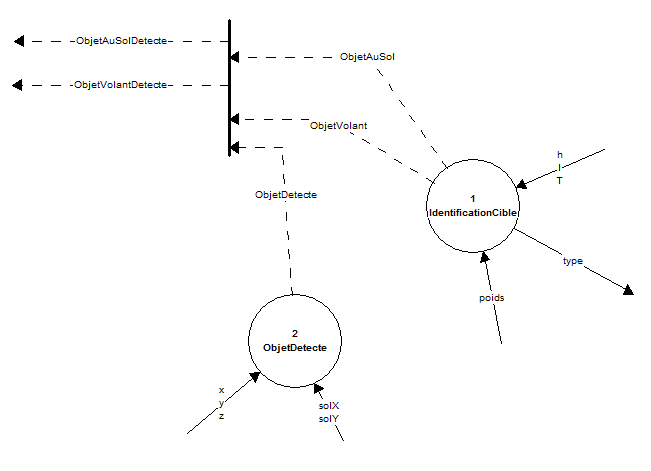
\includegraphics[height=11cm]{\PIXPATH/detecter}
\caption{Niveau 2 - Détecter}
\end{figure}
\end{center}


\subsubsection{Diagramme états-transitions}

\begin{center}
\begin{figure}[!h]
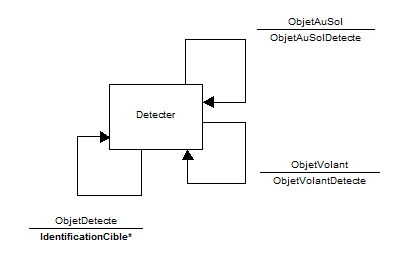
\includegraphics[height=6.5cm]{\PIXPATH/detecter_etat}
\caption{Diagramme états-transitions}
\end{figure}
\end{center}

\vfill
\pagebreak

\subsubsection{Processus primitifs - C-Spec}

\begin{description}
	
	\item \textbf{IdentificationCible}
		\begin{tabbing} 
		\textbf{IN} : h, l, T, poids \\
		\textbf{OUT} : poids, ObjetVolant, ObjetAuSol \\			
		/* Humain detecté */ \\
		si \=(h > 20 et l > 20 et T > 35) alors \\
			\>sortie \\
		fin si \\
		/* Rat detecté */ \\
		si (poids < 2.5 et T > 28) alors \\
			\>ObjetAuSolDetecte emis \\
		fin si \\
		/* Objet volant detecté */ \\
		si (h < 10 et l < 10 et T > 20) alors \\
			\>ObjetVolantDetecte emis \\
		fin si 
		\end{tabbing}
			

	\item \textbf{ObjetDetecte}
		\begin{tabbing} 
		\textbf{IN} : x, y, z, solX, solY \\
		\textbf{OUT} : ObjetDetecte \\
		si \=(x != 0 ou y != 0 ou z != 0 ou solX != 0 ou solY != 0) alors \\
		\>ObjetDetecte emis \\
		fin si
		\end{tabbing} 

\end{description}

\vfill
\pagebreak


